\documentclass[a4paper, 10pt, twocolumn]{article}

%\usepackage[colorlinks]{hyperref} % colored hyperlink
%\usepackage{adjustbox}
%\usepackage{amsmath}
%\usepackage{amssymb}
%\usepackage{amsthm}
%\usepackage[T1]{fontenc}
%\usepackage[french]{babel} % traduction
%\usepackage{blindtext}
%\usepackage{bookmark}
%\usepackage{booktabs} % beautiful tables
%\usepackage[thicklines]{cancel} % cancel terms in equation
%\usepackage{color}
\usepackage{csquotes}
%\usepackage{enumerate}
%\usepackage{framed} % box around text
%\usepackage{fancyhdr} % header
%\usepackage{fancyvrb}
\usepackage{lipsum}
%\usepackage{mathtools}
%\usepackage[parfill]{parskip}
%\usepackage{placeins}
%\usepackage{pgfplots} % plot in tikz
\usepackage[arrowdel]{physics} % physics helpers
%\usepackage{setspace}
\usepackage{siunitx}
%\usepackage{silence} % silence warnings
%\usepackage{systeme} % system of equations
\usepackage{tikz}
\usepackage{tkz-euclide}
\usepackage{tikz-3dplot}
\usepackage{units} % Non-stacked fractions and better unit spacing
%\usepackage[usenames,svgnames,dvipsnames]{xcolor}
%\usepackage{xspace} % prints a trailing space in a smart way.
\usepackage[backend=biber,style=apa,autocite=inline]{biblatex}
\DeclareLanguageMapping{french}{french-apa}

% \usetikzlibrary{calc,patterns,angles,quotes}

% \tikzset{circ/.style = {fill, circle, inner sep = 0, minimum size = 3}}
% \tikzset{scirc/.style = {fill, circle, inner sep = 0, minimum size = 1.5}}
% \tikzset{mstate/.style={circle, draw, blue, text=black, minimum width=0.7cm}}

\usepackage{enumitem}
\setlist{nosep,after=\vspace{\baselineskip}}

%\pgfplotsset{compat=1.12}
%\sisetup{locale = FR}

% \usepackage{graphicx}
% \setkeys{Gin}{width=\linewidth,totalheight=\textheight,keepaspectratio}
%\graphicspath{{figures/}}

% Default images settings
\setkeys{Gin}{width=\linewidth, totalheight=\textheight, keepaspectratio}

% conditions for equations
% https://tex.stackexchange.com/questions/95838/how-to-write-a-perfect-equation-parameters-description
\newenvironment{conditions}
  {\par\vspace{\abovedisplayskip}\noindent\begin{tabular}{>{$}l<{$} @{${}={}$} l}}
	{\end{tabular}\par\vspace{\belowdisplayskip}}

\newenvironment{conditions*}
  {\par\vspace{\abovedisplayskip}\noindent
   \tabularx{\columnwidth}{>{$}l<{$} @{${}={}$} >{\raggedright\arraybackslash}X}}
  {\endtabularx\par\vspace{\belowdisplayskip}}

%----------------
% FIX
%----------------

\setlength{\headheight}{14.5pt}

% increase vertical space for aligned equations
\setlength{\jot}{7pt}

% Filter warnings issued by package biblatex starting with "Patching footnotes failed"
%\WarningFilter{biblatex}{Patching footnotes failed}

%----------------------
%	COMMANDS
%----------------------

% commands shortcuts
\newcommand{\mb}{\mathbb}
\newcommand{\R}{\mb{R}}
\newcommand{\Z}{\mb{Z}}
\newcommand{\N}{\mb{N}}
\newcommand{\C}{\mb{C}}
\newcommand{\dS}{\cdot d\vec{S}}
\newcommand{\lag}{\mathcal{L}}
\newcommand{\vd}[1]{\dot{\va{#1}}}
\newcommand{\vdd}[1]{\ddot{\va{#1}}}

% big norm
\newcommand{\bignorm}[1]{\left\lVert#1\right\rVert}

% prints an asterisk that takes up no horizontal space.
% useful in tabular environments.
\newcommand{\hangstar}{\makebox[0pt][l]{*}}

% Prints argument within hanging parentheses (i.e., parentheses that take
% up no horizontal space). Useful in tabular environments.
\newcommand{\hangp}[1]{\makebox[0pt][r]{(}#1\makebox[0pt][l]{)}}

% cancel terms with color
%\newcommand{\ccancel}[2]{\renewcommand{\CancelColor}{\color{#2}}\bcancel{#1}}

\renewcommand*\contentsname{Table des matières}

%-----------------
% HEADER / FOOTER
%-----------------

% header
\chead{\textit{\ntitle}}

% footer
\rfoot{\footnotesize Page \npage\ \\ pageref{LastPage}}

% page style for the first page
\fancypagestyle{firstpage}{
  \fancyhf{}
  \renewcommand{\footrulewidth}{0.0pt} % no footer rule
}

%----------
% TITLE
%----------

% custom title
\usepackage{titling} % Allows custom title configuration

% Gold horizontal line around the title
\newcommand{\HorRule}{\color{DarkGoldenrod}\rule{\linewidth}{1pt}}

% custom title
\pretitle{
	\vspace{-30pt} % Move the entire title section up
	\HorRule\vspace{10pt} % Horizontal rule before the title
	\fontsize{32}{36}\usefont{OT1}{phv}{b}{n}\selectfont % Helvetica
	\color{DarkRed} % Text colour for the title and author(s)
}

\posttitle{\par\vskip 15pt} % Whitespace under the title

\preauthor{} % Anything that will appear before \author is printed

\postauthor{ % Anything that will appear after \author is printed
	\vspace{10pt} % Space before the rule
	\par\HorRule % Horizontal rule after the title
	\vspace{20pt} % Space after the title section
}

%--------------------------
% AUTHORS AND INSTITUTIONS
%--------------------------

% author
\newcommand{\authorstyle}[1]{{\large\usefont{OT1}{phv}{b}{n}\color{DarkRed}#1}} % Authors style (Helvetica)

% institution
%\newcommand{\institution}[1]{{\footnotesize\usefont{OT1}{phv}{m}{sl}\color{Black}#1}} % Institutions style (Helvetica)

%----------
% ABSTRACT
%----------

\usepackage{lettrine} % Package to accentuate the first letter of the text (lettrine)
\usepackage{fix-cm}	% Fixes the height of the lettrine

\newcommand{\initial}[1]{ % Defines the command and style for the lettrine
	\lettrine[lines=3,findent=4pt,nindent=0pt]{% Lettrine takes up 3 lines, the text to the right of it is indented 4pt and further indenting of lines 2+ is stopped
		\color{DarkGoldenrod}% Lettrine colour
		{#1}% The letter
	}{}%
}

\usepackage{xstring} % Required for string manipulation

\newcommand{\lettrineabstract}[1]{
	\StrLeft{#1}{1}[\firstletter] % Capture the first letter of the abstract for the lettrine
	\initial{\firstletter}\textbf{\StrGobbleLeft{#1}{1}} % Print the abstract with the first letter as a lettrine and the rest in bold
}

%--------------
% BIBLIOGRAPHY
%--------------
\usepackage[backend=biber,style=apa,autocite=inline]{biblatex}
\DeclareLanguageMapping{french}{french-apa}
\usepackage[autostyle=true]{csquotes} % Required to generate language-dependent quotes in the bibliography


\title{Étude de la bifurcation de fold-hopf en tant que point de cascade dans le système climatique}
\author{
  \authorstyle{Mathieu Rousseau\textsuperscript{1}}
  \newline\newline % space before institution
  \textsuperscript{1}\institution{Université catholique de Louvain, École de Physique, Louvain-La-Neuve. Belgique}
}
%\author[1] {Mathieu Rousseau}

%\affil[1] {Université Catholique de Louvain, Ecole de Physique, Louvain-La-Neuve, Belgique}

% \def\npromotor {Michel Crucifix}
% \def\ndate {\today}

%% Université Catholique de Louvain %%
%% Faculté des Sciences %%
%% Ecole de Physique %%
%% 2020-2021 %%

%\runningauthor{Rousseau}
\addbibresource{references.bib}

\begin{document}

% \showthe\textwidth
% \showthe\columnwidth

\maketitle
\thispagestyle{firstpage}

% \begin{abstract}
%   \lipsum[1]
%   \keywords{Système climatique, Points de cascade, Bifurcation fold-hopf, Dynamique non-linéaire}
% \end{abstract}

\lettrineabstract{\lipsum[1]}

\section{Introduction}

Notre planète subit un changement climatique, il fut un temps où politiques, économistes et même scientifiques ont pensé que le changement climatique induit par l'homme était prédictible et que ses conséquences apparaitraient graduellement, linéairement dans le temps. Pourtant plusieurs recherches ont mis en évidence la possible existence de \emph{points de bascules} dans le système climatique (\cite{lenton_tipping_2008}). Il s'agit d'un changement apparaissant dans un sous-système climatique (dû à la monter des températures par exemple) induisant un changement dans un autre sous-systèmes climatiques. Si l'on se représente le système climatique terrestre comme un \emph{système dynamique} alors on peut voir ce point de bascule comme une bifurcation. Il s'agit d'un changement structurelle dans le système lorsqu'un paramètre $\phi$ de ce système atteint une valeur critique $\phi_c$. Alors qu'on approche ces points de bascule à un temps $t$, un petit changement peut suffir à passer ces points critiques et avoir de graves conséquences. Cela peut notamment induire des boucles de rétroactions positives (qui empirent un changement climatique par exemple) ou encore des bifurcations où le comportement future du système devient instable. D'ailleurs ces transitions peuvent être brusque, irréversibles ou même parfois les deux. Par exemple TODO: exemples de l'Arctique (\cite{Lenton_2012}). A titre d'exemple de points de cascade nous pourrions citer la banquise Arctique, la circulation thermohaline Atlantique ou encore la Forêt Boréal (\cite{lenton_tipping_2008}). Des recherches récentes (TODO: sources) montrent que des signes indiqueraient que ces points de bascules soient plus probables qu'il était pensé autrefois et qu'ils impliqueraient des changements irréversibles (\cite{lenton_climate_2019_too_risky}). Dès lors, ces points de bascules constituent une urgence climatique d'autant plus que des récents rapports de l'IPCC parus en 2018 et 2019 suggèrent qu'un réchauffement de 1 à \SI{2}{\celsius} suffirait à dépasser ces points (\cite{ipcc_global_2018,portner_ipcc_2019}). Pire encore, on serait proche de certains points de bascules et certains sous-sytèmes climatiques auraient déjà passé un point de cascade à l'image par exemple de l'échancrure de la mer d'Amundsen en Antarctique Ouest (\cite{portner_ipcc_2019}) où la ligne de rencontre de la glace, la roche et l'océan est en train de reculer de façon irréversible ce qui pourrait déstabiliser le reste de la calotte glaciaire (de l'Antarctique Ouest) par effet domino (\cite{feldmann_collapse_2015_amundsen}). La conséquence est sans appel, un montée du niveau d'eau d'environ 3m s'étalant sur plusieurs centaines voire milliers d'années. Ces points de bascules font peut-être partie des plus grandes menaces climatiques.

L'objectif de cet article est de s'intéresser aux points de bascules en tant que bifurcations et plus particulièrement d'étudier la bifurcation \emph{fold-hopf} et quelles seraient les conséquences pour un système climatique passant cette bifurcation. Premièrement on définit la théorie des systèmes dynamiques derrière cette bifurcation. Ensuite on analyse les bifurcations de fold et hopf à elles seules et leurs conséquences pour ensuite les coupler et former la bifurcation fold-hopf. Par après on regarde comment cette bifurcation se passe dans le temps. Enfin, on ajoute du bruit à notre système dynamique et regardons ses conséquences.

\section{Bifurcation de fold-hopf}

Pour qu'un système soit qualifié d'élément de bascule, il doit être possible d'y identifier un paramètre de forçage $\phi$ pour lequel il existe une certaine valeur critique $\phi_c$ tel qu'une petite perturbation $\delta \phi$ induise un changement qualitatif dans la structure du système.
Cette bifurcation apparaît dans un système d'équations différentielles ordinaires (EDOs) $f: \Omega \subseteq \R^n \rightarrow \R^n$ constitué à la fois d'une EDO sur la droite ($\Omega = \R$) et d'un système d'EDOs dans le plan ($\Omega = \R^2$) que l'on appellera système secondaire. De ce premier système surgit deux bifurcations de type \emph{"Fold"} tandis que du second système surgit une bifurcation de type \emph{"Hopf"}.

Nous considérerons le système suivant,
\begin{equation} \label{eq:fold-hopf}
  \begin{cases}
    \dot{x} = a_1x^3 + a_2x + \phi \\
    \dot{y} = b_1z + b_2(\gamma(x) - (y^2 + z^2))y \\
    \dot{z} = c_1y + c_2(\gamma(x) - (y^2 + z^2))z
  \end{cases}
\end{equation}
où $\phi$ est un paramètre de forçage et $\gamma(x) = \gamma_1 + \gamma_2 x$ est un paramètre de couplage linéaire.
Nous appellerons $\dot{x}$ le \textbf{système primaire} et l'ensemble $\dot{y}$ et $\dot{z}$ le \textbf{système secondaire}.

Alors que nous nous approchons de la valeur critique de la bifurcation que nous noterons $\phi_{c}$, une petite perturbation du paramètre $\phi$ suffit pour passer la bifurcation et modifier considérablement le comportement qualitatif du système. Dans le langage des systèmes dynamiques on dit qu'il y a création, suppression d'équilibres voir modification dans la nature de ces équilibres. Toutefois, dans la définition des points de bascules, il en existe certains qui sont réversibles et qui ne sont donc pas dû à des bifurcations (\cite{lenton_tipping_2008}). Nous ne considérerons pas ces derniers dans cet article.

\subsection{Bifurcation fold} \label{sec:fold}

\begin{figure*}[htbp]
  \centering
  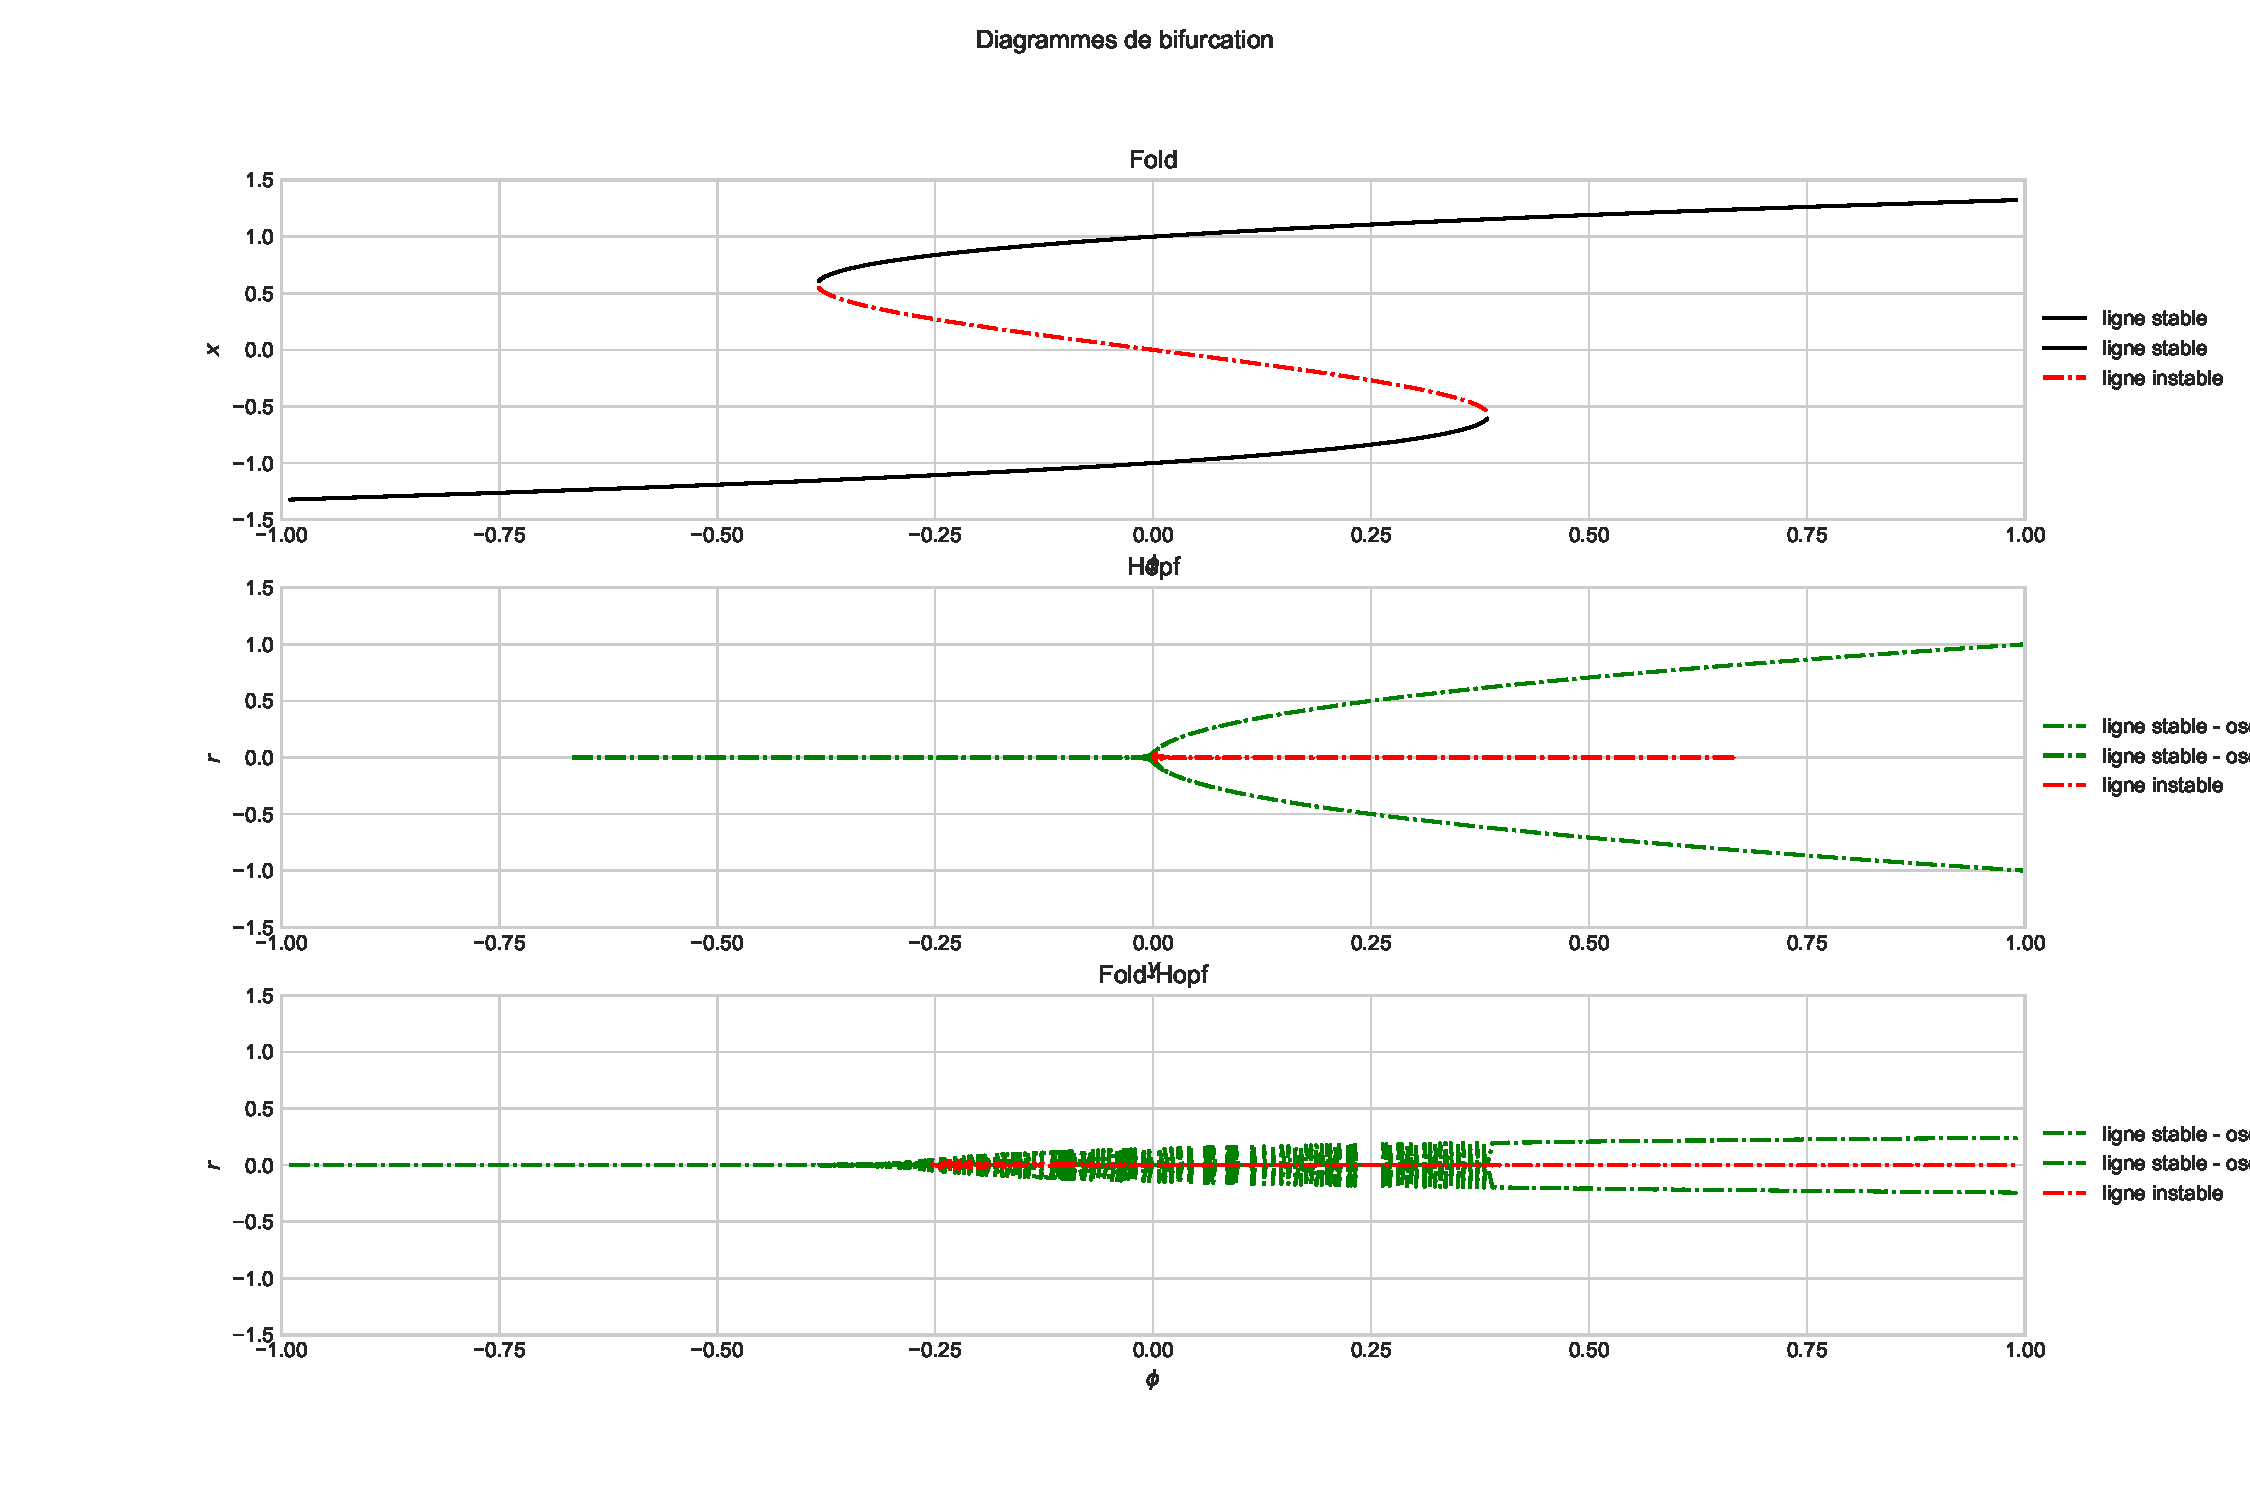
\includegraphics{figures/bifurcations.pdf}
  \caption{(a) Système primaire vs forçage $\phi$. (b) Système secondaire vs couplage $\gamma$. (c) Système secondaire vs forçage $\phi$. Les lignes noires correspondent aux équilibres stables tandis que les lignes rouges en traits pointillés correspondent aux équilibres instables. Les lignes vertes en traits pointillés correspondent à des équilibres stables avec un régime oscillatoire. Les points rouges sont les points de bascule de la bifurcation fold tandis que les points oranges sont les points de bascules de la bifurcation de hopf.}
  \label{fig:bifurcations}
\end{figure*}

Considérons le système primaire,
\begin{equation} \label{eq:fold}
  \dot{x}(t) = a_1 x^3 + a_2 x + \phi \equiv f_{\phi}(x),  \quad a_1, a_2 \in \R
\end{equation}
Cette équation fait apparaître une bifurcation fork qui est une combinaison de 2 bifurcations points de selle. Une bifurcation point de selle consiste en l'apparition de 2 équilibres, un stable et un instable lorsqu'on atteint une certaine valeur de $\phi$. La bifurcation fork consiste en l'apparition de 3 équilibres, 2 stables et 1 instable lorsque $\phi$ se trouve dans une certaine intervalle induisant alors une bistabilité. Dans le cas de ce système, cette dernière se trouve dans l'intervalle
\begin{equation} \label{eq:phi_c-range}
  |\phi_c| < \sqrt{\frac{-4(a_2)^3}{27a_1}}
\end{equation}
où $a_1 < 0 < a_2$ ou $a_1 > 0 > a_2$.

Pour des valeurs de paramètres cités dans le tableau (\ref{tab:basic-parameters}) cette intervalle vaut $]-0.38, 0.38[$.
Cette bifurcation a la particularité de présenter un phénomène dit \emph{d'hystérésis} c'est à dire que le système se comporte à la fois selon la valeur courante du paramètre de forçage mais également selon son historique.

Le système a un ou plusieurs points d'équilibres en $x = x_0$ lorsque $f_{\phi}(x_0) = 0$. On peut voir cette EDO comme la somme de 2 courbes, $f_1(x) = a_1 x^3$ et $f_2(x) = - (a_2x + \phi_c)$. Les équilibres du système correspondent aux points d'intersection de $f_1$ et $f_2$. Si l'on trace ces 2 fonctions, on remarque la création de 2 équilibres lorsque la droite $f_2$ est tangente à la fonction cubique $f_1$. On peut de par cette observation facilement repérer nos points d'équilibres
\begin{equation}
  f_{\phi_c}'(x_0) = 0 \implies x_0 = \pm \sqrt{-\frac{a_2}{3a_1}}
\end{equation}

L'analyse graphique nous montre qu'il s'agit de 2 équilibres stables. Il existe également un équilibre instable situé entre ces 2 derniers.
Si l'on injecte cette valeur de $x_0$ dans l'équation pour la condition d'équilibre du système $f_{\phi}(x_0) = 0$, on trouve après un peu d'algèbre la condition (\ref{eq:phi_c-range}).

% TODO: trouver mathématiquement l'équilibre instable x_0^(instable)

On peut mieux se rendre compte de la dynamique du système en traçant son diagramme de bifurcation (\autoref{fig:bifurcations}a),

Lorsqu'on approche $\phi_c$ par des valeurs $\phi < \phi_c$, le système est dans un état stable. Une fois que l'on atteint $\phi_c$ (dans le système climatique il pourrait s'agit d'une température critique, une concentration de CO2 critique,\dots), le système est attiré vers un nouvel état stable (branche supérieur de la \autoref{fig:bifurcations}a). Si le paramètre de forçage continue d'augmenter, le système reste stable. Par contre si un quelconque phénomène arrivait à baisser la valeur de $\phi$ jusqu'à la valeur $-\phi_c$, le système repasserait dans l'état stable initial. On voit que ré-augmenter la valeur du paramètre de forçage la transition critique faite ne fait pas directement repasser le système dans son état initial. Il s'agit bien là d'un phénomène d'hystérésis. Un raisonnement analogue peut être fait si l'on approche $-\phi_c$ par des valeurs $\phi > -\phi_c$. Toutefois, entre ces 2 branches stables existent une branche instable. Dès lors, lorsque la valeur du paramètre de forçage se trouve dans l'intervalle critique, le système se verra dans un des 2 états stables dépendant des conditions initiales (les solutions du systèmes convergeront vers la branche haute (\emph{resp. basse}) si la condition initiale $x_0$ est supérieure (\emph{resp. inférieure}) à la valeur de l'équilibre instable pour un $\phi_0$ donné appartenant à l'intervalle critique). Il est également possible que des conditions initiales fassent que le système se situe sur la courbe instable mais du fait de la nature de cet équilibre, une perturbation des conditions initiales amènerait le système à être attiré vers une des branches stables.

\subsection{Bifurcation hopf (supercritique)}

Considérons le système secondaire et remplaçons le paramètre de couplage $\gamma(x)$ par un paramètre de forçage $\gamma$.
\begin{equation} \label{eq:hopf}
  \begin{cases}
    \dot{y} = b_1z + b_2(\gamma - (y^2 + z^2))y \equiv f_{1,\gamma}(y,z) \\
    \dot{z} = c_1y + c_2(\gamma - (y^2 + z^2))z \equiv f_{2, \gamma}(y,z)
  \end{cases}
\end{equation}
où $b_1, b_2, c_1, c_2 \in \R$.

Les points d'équilibre sont $x = 0$ et $y = 0$ si $c_1 > 0$. Nous avons également les condition $b_2c_2 < 0$ et $b_1 > 0$.
% Afin de trouver la nature de ces équilibres, on peut analyser les valeurs propres la matrice jacobienne $df$ au point d'équilibre $\vb{p} = (0, 0)$.

Sans perte de généralité, posons $b_1 = b_2 = 1$, $c_1 = -1$ et $c_2 = 1$.
% \begin{equation}
%   df(\vb{p}) =
%   \begin{pmatrix}
%     \gamma & 1 \\
%     -1 & \gamma
%   \end{pmatrix}
% \end{equation}

% %TODO: valeurs propres

Afin de mieux comprendre la façon de se comporte notre système, on peut passer en coordonnées polaires $(r, \theta)$
\begin{equation}
  \begin{cases}
    \dot{r} = \gamma r - r^3 \\
    \dot{\theta} = -1
  \end{cases}
\end{equation}

L'analyse graphique de l'équation pour $\dot{r}$ nous montre la présence d'un équilibre stable en $r = 0$ pour $\gamma < 0$ par contre lorsque $\gamma \geq 0$, l'équilibre en $r = 0$ devient instable et il apparaît un nouvel attracteur en $r = \sqrt{\gamma}$. Il y a à la fois changement dans la nature d'un équilibre et création d'un autre équilibre. On comprend donc que lorsque $\gamma \geq 0$ il apparaît un cycle limite de rayon $r = \sqrt{\gamma}$ où toutes les solutions partant en dehors de ce cycle y convergent. C'est ce que nous voyons sur la figure (\ref{fig:bifurcations}b) Ce cycle limite stable apparaît en une valeur de $\gamma$ supérieure à celle du point d'équilibre instable. On nomme alors cette bifurcation une bifurcation de hopf \emph{supercritique}.

\subsection{Bifurcation fold-hopf}

Le système que nous étudions présente un mix de ces 2 bifurcations. L'équation pour $\dot{x}$ donne lieu à une bifurcation fold tel que nous l'avons vue à la section (\ref{sec:fold}). L'équation pour $\dot{y}$ et $\dot{z}$ est un peu différente dans le sens où nous considérons dès à présent un paramètre de couplage $\gamma(x)$ qui dépend de la première équation. Par ailleurs, nous supposerons lorsque nous élaborerons la série temporelle du système que $\phi = \phi(t)$ varie lentement en fonction du temps.

% BIFURCATION

Imaginons que l’on parte d’une valeur de $\phi < - \phi_c$. Si l’on augmente lentement le paramètre de forçage $\phi$ dans la branche basse du système primaire, une fois atteint une valeur $-\phi_c$, le système primaire entre dans son régime bistable où les solutions convergeront vers l’une des 2 branches stables du système dépendant de leurs conditions initiales. Une fois atteint $+\phi_c$, on quitte le régime bistable et toutes les solutions convergerons vers la branche stable supérieure. Une fois passé $\phi_c$, la valeur de $x$ augmente de manière conséquente comparé à son augmentation négligeable lorsque $+\phi$ se situe dans l’intervalle $]-\infty, +\phi_c[$ ce qui a pour conséquence d’augmenter significativement le paramètre de couplage $\gamma(x)$ présent dans le système secondaire. Le système génère alors par cascade un cycle limite caractérisant des solutions oscillantes où toutes les solutions convergent vers ce cycle peut importe leurs conditions initiales.

\begin{figure*}[ht!]
  \centering
  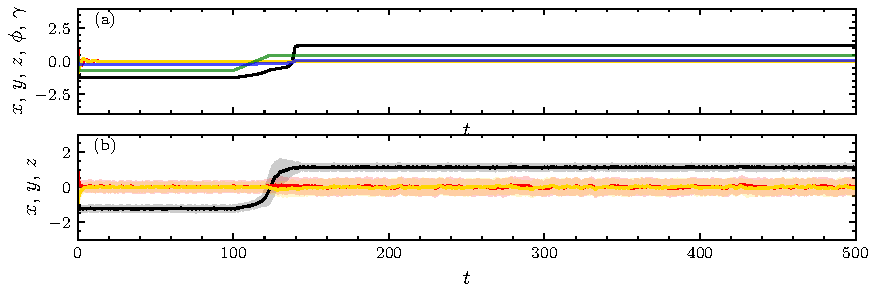
\includegraphics{figures/time-series.pdf}
  \caption{(a) Série temporelle sans bruit. (b) Série temporelle bruitée contenant un ensemble de 100 simulations avec un terme stochastique. Dans cette dernière, les lignes correspondent aux moyennes des différents états du systèmes correspondants tandis que les zones de faible opacités correspondent aux déviations standards $[\mu - \sigma, \mu + \sigma]$ des états correspondants. La ligne noire correspond au système primaire. Les lignes jaunes et rouges correspondent au système secondaire. La ligne verte est la valeur du paramètre de forçage $\phi$ et la ligne bleue est la valeur du paramètre de couplage $\gamma(x)$.}
  \label{fig:time-series}
\end{figure*}

C'est précisément ce que l'on peut remarquer sur la figure (\ref{fig:bifurcations}c). Lorsqu'on se situe dans l'intervalle $]-\infty, -\phi_c[$, le système primaire n'a qu'un seul point d'équilibre négatif ce qui pour conséquence de laisser le système secondaire dans son état stable. Pour $\phi \in ]-\phi_c, +\phi_c[$, le système primaire a 3 positions d'équilibre. Pour chaque $\phi$ appartenant à cette intervalle, la plus haute valeur des 3 points d'équilibre est toujours positive et en constante augmentation alors que $\phi$ augmente. Nécessairement, le système secondaire ne tardera pas à passer son point de bascule à partir de valeurs de $\phi$ égalent à $-\phi_c + \delta \phi \equiv \phi_{ast}$. Toutefois, pour les 2 autres points d'équilibres du premier système, le système secondaire restera dans son état stable. Il y a alors coexistence d'états stables et oscillatoires à partir de cette valeur de $\phi_{ast}$. Enfin, une fois atteint l'intervalle $]\phi_c, +\infty[$, le système primaire n'a à nouveau plus qu'un seul équilibre dont sa valeur est plus grande que la plus grande valeur du triplet d'équilibre de l'intervalle $]-\phi_c, +\phi_c$ pour chaque $\phi$ ce qui a pour conséquence de pousser le système secondaire uniquement dans son état où nous avons à la fois toujours 2 branches stables oscillatoires mais également une branche instable. Une représentation temporelle d'une telle cascade de bifurcations se situe sur la figure (\ref{fig:time-series}a).

Un cas où une telle bifurcation pourrait éventuellement arriver serait le cas où un effondrement de la circulation méridionale de retournement de l'Atlantique (AMOC)\footnote{Désigne l'ensemble des courants océaniques (Gulf stream, circulation thermohaline,...) régissant les échanges de chaleur entre l'équateur et les pôles.} entraînerait un renforcement ou un affaiblissement du phénomène El-Niño\footnote{Phénomène climatique caractérisé par des températures anormalement élevées de l'eau dans la partie Est de l'océan Pacifique-Sud} \cite{timmermann_influence_2007}. Ici, l'effondrement de l'AMOC correspond au passage de la branche basse à la branche haute dans la bifurcation fold (figure \ref{fig:bifurcations}a). Tandis le renforcement / affaiblissement de El-Niño correspond aux 2 branches oscillatoires dans la bifurcation hopf (figure \ref{fig:bifurcations}b). Le retournement est lui forcé par le flux d'eau douce et donc ce dernier correspond au paramètre $\phi$ tandis que le couplage avec l'Océan Pacifique est assuré par les alizés\footnote{Vent régulier des régions intertropicales soufflant d'Est en Ouest de façon régulière à partir des hautes pressions subtropicales vers les basses pressions équatoriales} et correspond au paramètre $\gamma$.

% SERIES TEMPORELLES

On a vu que la transition dans le système secondaire est générée par cascade une fois que le système primaire à passé son point critique $\phi_c$. En particulier nous avons vu que la transition de ce dernier induit un "grand saut" dans la variable $x$ ce qui a pour conséquence de fortement augmenté le paramètre de couplage et donc de pousser le système secondaire à passer son point critique. Tout cela rend le système secondaire fortement dépendent de la bifurcation du système primaire.
On peut dès à présent considérer le système (\ref{eq:fold-hopf}) où nous ajoutons un terme stochastique $\xi_i$ avec $i \in \{x, y, z\}$. Il s'agit en réalité de bruit blanc gaussien. Ce bruit peut également pousser le système à passer un point de bifurcation.
Au préalable de cette bifurcation, le système secondaire est peu dépendant du système primaire et plus sensible au bruit. En effet, un système dynamique stochastique est caractérisé par un ralentissement de ses fluctuations lorsqu'un point critique est approché (figure \ref{fig:time-series}) ce qui a pour conséquence d'augmenter l'auto-corrélation et la variance. Ceci est particulièrement vrai pour la bifurcation fold dû à son irréversibilité (\emph{hystérésis}) et son changement d'état brusque. On remarque qu'au démarrage de la série temporelle stochastique, le système secondaire atteint directement son point d'équilibre $(x,y) = (0,0)$ (alors qu'il oscille pendant quelques temps dans la simulation non-stochastique) tandis que le système primaire est dans un état stable. Alors que le système primaire approche son point de bascule via le forçage $\phi(t)$, sa variance augmente (on peut le voir par l'augmentation de la dispersion en gris clair autour de la moyenne). Par la suite lorsqu'il bascule, le bruit induit par cette bascule pousse le système secondaire à passer son point critique et à basculer directement.

\section{Conclusion}

Après avoir introduit le concept de points de bascule et leur importance cruciale dans l'étude du système climatique, en considérant le système climatique comme un grand système dynamique nous avons vu que nous pouvions modéliser des sous-systèmes climatiques sous forme d'équations différentielles ordinaires. Nous nous sommes concentrés en particulier sur un système induisant une bifurcation de fold-hopf. Nous avons vu que l'on pouvait décomposer ce système en un système primaire et secondaire et que ces deux derniers étaient alors couplés par un paramètre de couplage $\gamma(x)$. En faisant lentement varier le paramètre de forçage $\phi$ dans le système primaire on a alors vu que la bascule de ce dernier induisait la bascule du second par cascade et ainsi la coexistence d'états stables et oscillatoires. On a finalement regardé ce qu'il se passait lorsqu'on introduisait un terme stochastique au système. Nous avons remarqué que cette bifurcation pourrait éventuellement apparaître dans un modèle décrivant le lient entre l'AMOC et le phénomène El-Niño. Un modélisation simple de ce phénomène est disponible dans l'article de \cite{dekker_cascading_2018}. Toutefois, il s'agit d'un modèle fortement idéalisé et de plus amples recherches sur des modèles plus détaillés sont nécessaires afin de démontrer si de telles bascules sont possibles dans le système climatique.

Comme nous l'avons mentionné en introduction, plusieurs recherches ont mis en évidence la possible existence de points de bascules. Au vu de l'importance et des conséquences de ces derniers sur notre climat et à fortiori sur notre société, ce sujet est d'une importance cruciale et de plus amples recherches sont dès lors nécessaires.



\newpage

%\bibliographystyle{agu}
%\bibliography{references}
%\nocite{*}
\printbibliography
\nocite{*}

\newpage

\appendix
\appendixpage
\addappheadtotoc
\section{Intervalle critique dans la bifurcation de fold}
Soit l'EDO à 1 paramètre
\begin{equation}
  \dot{x}(t) = a_1x^3 + a_2x + \phi \equiv f_{\phi}(x), \quad a_1, a_2 \in \R
\end{equation}
On peut la voir comme la somme d'une fonction cubique et d'une droite. En traçant les 2 graphes, on observe que nous avons plusieurs équilibres pour $a_1 < 0 < a_2$ ou $a_2 < 0 < a_1$. Il existe au moins un équilibre lorsque la droite et la fonction cubique s'intersectent.
\begin{equation} \label{eq:intersection}
  f_{\phi_c}(x_0) = 0 \iff a_1 x_0^3 = - (a_2x_0 + \phi_c)
\end{equation}
Il y a création de 3 équilibres lorsque la droite est tangente à la fonction cubique.
\begin{align*}
  f'_{\phi_c(x_0)} = 0
    &\iff a_1x_0^3 = -a_2 \\
    &\iff x_0^2 = - \frac{a_2}{3a_1} \\
    &\iff x_0 = \pm \sqrt{- \frac{a_2}{3a_1}}
\end{align*}
ce qui implique en injectant dans (\ref{eq:intersection}) que
\begin{align*}
  \pm a_1 \left( - \frac{a_2}{3a_1} \right)^{3/2}
    &= - \left( \pm a_2 \left[ - \frac{a_2}{3a_1} \right]^{1/2} + \phi_c \right) \\
  \iff \phi_c
    &= \mp a_1 \left( - \frac{a_2}{3a_1} \right)^{3/2} \mp a_2 \left( - \frac{a_2}{3a_1} \right)^{1/2} \\
    &= \mp a_1 \left( - \frac{a_2}{3a_1} \right)^{3/2} \mp a_2 \left( - \frac{a_2}{3a_1} \right)^{1/2} \frac{3}{3} \\
    &= \pm \frac{4(-a_2)^{3/2}}{(27a_1)^{1/2}}
\end{align*}

On a donc trouvé l'intervalle critique où il y a création 3 équilibres.
\begin{equation}
  |\phi_c| < \sqrt{\frac{-4(a_2)^3}{27a_1}}
\end{equation}
pour $a_1 < 0 < a_2$ ou $a_2 < 0 < a_1$.

% \section{La bifurcation de Hopf a un unique équilibre en $(y,z)=(0,0)$}
% Soit le système d'EDO,
% \begin{equation}
%   \begin{cases}
%     \dot{y} = b_1z + b_2[\gamma - (y^2 + z^2)]y \equiv f_{1,\gamma}(y,z) \\
%     \dot{z} = c_1y + c_2[\gamma - (y^2 + z^2)]z \equiv f_{2,\gamma}(y,z)
%   \end{cases}
% \end{equation}
% avec $b_1, b_2, c_1, c_2 \in \R_{\ast}$.

% Il y a équilibre lorsque $\vb{f}_{\gamma}(y,z) = 0$ c'est à dire,
% \begin{align*}
%   \vb{f}_{\gamma}(y,z) = 0
%     &\iff
%   \begin{cases}
%     0 &= b_1z + b_2[\gamma - (y^2 + z^2)]y \\
%     0 &= c_1y + c_2[\gamma - (y^2 + z^2)]z
%   \end{cases} \\
%     &\implies
%   \begin{cases}
%     b_1z &= b_2[\gamma - (y^2 + z^2)]y \\
%     0 &= c_1y + c_2[\gamma - (y^2 + z^2)]^2 \frac{b_2}{b_1} y
%   \end{cases}
% \end{align*}

% On trouve donc,
% \begin{equation*}
%   0 = y \left( c_1 - c_2 \frac{b_2}{b_1} \underbrace{[\gamma - (y^2 + z^2)]^2}_{\equiv \eta} \right)
% \end{equation*}

% Ce qui implique que $y = 0$ si $c_1 \neq c_2 \frac{b_2}{b_1}$.

% Si $y = 0$ alors $z = 0$ et $(y,z) = (0,0)$ est le seul équilibre réel de ce système.

\section{Le système secondaire avec paramètre de forçage a un cycle limite}

Sans perte de généralités, posons $b_1 = b_2 = 1$ et $c_1 = -1$ et $c_2 = 1$.

Le système (\ref{eq:hopf}) devient,
\begin{equation}
  \begin{cases}
    \dot{y} &= 1z + 1[\gamma - (y^2 + z^2)]y \\
    \dot{z} &= -1y + 1[\gamma - (y^2 + z^2)]z
  \end{cases}
\end{equation}
Passons en coordonnées polaires $(r, \theta)$\footnote{On retrouve facilement les relations de changement de coordonnées en dérivant $r^2 = y^2 + z^2$ et $\theta = \arctan(z/y)$}.
\begin{align*}
  \dot{r} = \frac{y\dot{y} + z\dot{z}}{r}
    &= \frac{y(z + \gamma y - r^2 y) + z(-y + \gamma z - r^2 z)}{r} \\
    &= \frac{\gamma y^2 + \gamma z^2(y^2 + z^2)}{r} \\
    &= \frac{\gamma r^2 - r^4}{r} \\
    &= \gamma r - r^3 \equiv f_r(\gamma)
\end{align*}
\begin{align*}
  \dot{\theta} = \frac{\dot{z}y - z\dot{y}}{r^2}
    &= \frac{(-y + \gamma z - r^2 z)y - z(z + \gamma y - r^2 y)}{r^2} \\
    &= \frac{- y^2 - z^2}{r^2} \\
    &= -1
\end{align*}
L'EDO est $\dot{\theta}$ est facilement résolvable par séparation des variables. On trouve $\theta = -t + \theta_0$. L'analyse graphique de l'équation pour $\dot{r}$ nous renseigne sur la nature des équilibres de cette dernière.
On trouve en effet aisément que cette EDO a des équilibres en $r = 0$ pour tout $\gamma \in \R$ et $r = \sqrt{\gamma}$ pour $\gamma \geq 0$.

L'analyse graphique nous montre que,
\begin{itemize}
  \item pour $\gamma < 0$, l'équilibre en $r = 0$ est un attracteur.
  \item pour $\gamma \geq 0$, l'équilibre en $r = 0$ est une source et $r = \sqrt{\gamma}$ est un attracteur.
\end{itemize}

Cela nous montre bien l'apparition d'un cycle limite dans le plan $(y,z)$ pour des valeurs de $\gamma \geq 0$.

L'équation pour $\dot{\theta}$ nous montre que les trajectoires ont un sens horloger (autour de l'origine) tandis que l'équation paramétrique de ce cycle limite est donnée par,
\begin{equation}
  \begin{cases}
    y &= \sqrt{\gamma} \sin(\theta_0 - t) \\
    z &= \sqrt{\gamma} \cos(\theta_0 - t)
  \end{cases}
\end{equation}

Ci-dessous le portrait de phase du système $(\ref{eq:hopf})$ pour $\gamma = 1$. On voit bien les solutions converger vers ce cycle.
\begin{figure}[H]
  \centering
  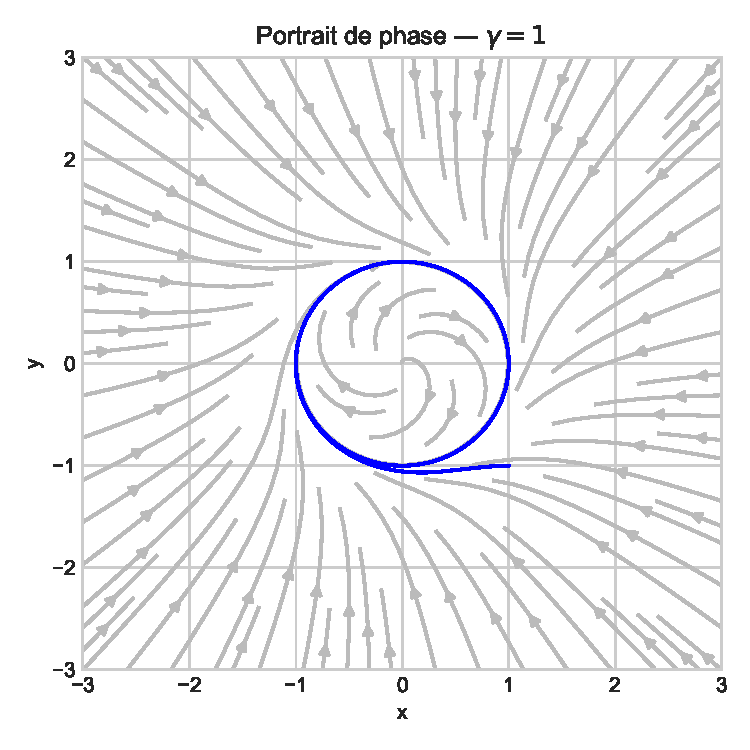
\includegraphics{figures/phase-plot.pdf}
  \caption{Portrait de phase du système d'équations différentielles (\ref{eq:hopf}) pour $\gamma = 1$. Le cycle limite est affiché en bleu.}
  \label{fig:phase-plot}
\end{figure}

\section{Paramètre utilisés dans les simulations}
\begin{table}[H]
\centering
\begin{tabular}{lcc} \toprule
  & \multicolumn {2}{c}{Valeur} \\\cmidrule(lr) {2-3}
  Paramètre         & Non-Stochastique                & Stochastique\\\hline
  $\phi(t)$         & $0.5t$                          & $0.5t$ \\
  $\gamma_1$        & $-0.1$                          & $-0.2$ \\
  $\gamma_2$        & $0.12$                          & $0.3$ \\
  $a_1$             & $-1$                            & $-1$ \\
  $a_2$             & $1$                             & $1$ \\
  $b_1$             & $1$                             & $0.1$ \\
  $b_2$             & $1$                             & $1$ \\
  $c_1$             & $-1$                            & $-0.5$ \\
  $c_2$             & $1$                             & $1$ \\
  $t$               & $[0, 500]$                      & $[0, 500]$ \\
  $\Delta t$        & $0.2$                           & $0.1$ \\
  $(x_0, y_0, z_0)$ & $(-0.5, 1, -1)$                 & $(-0.5, 1, -1)$ \\
  $Moyenne$         & //                              & $0$ \\
  $Variance$        & //                              & $0.1$ \\\hline
\end{tabular}
\caption{Au centre, les paramètres utilisés dans les différentes bifurcation et la série temporelle non stochastique. A droite, les paramètres utilisés dans la série temporelle stochastique}
\label{tab:parameters}
\end{table}


\end{document}
